%----------------------------------------------------------------------------------------
%	PACKAGES AND OTHER DOCUMENT CONFIGURATIONS
%----------------------------------------------------------------------------------------

\documentclass{article}

\usepackage{fancyhdr} % Required for custom headers
\usepackage{lastpage} % Required to determine the last page for the footer
\usepackage{extramarks} % Required for headers and footers
\usepackage[usenames,dvipsnames]{color} % Required for custom colors
\usepackage{pgf} % Required to insert pgf plots from matplotlib
\usepackage{graphicx} % Required to insert images
\usepackage{listings} % Required for insertion of code
\usepackage{courier} % Required for the courier font
\usepackage{lipsum} % Used for inserting dummy 'Lorem ipsum' text into the template
\usepackage[utf8]{inputenc}
\usepackage[ngerman]{babel}
\usepackage{subcaption, caption, tabularx, minted}
\usepackage{hyperref}

% Margins
\topmargin=-0.45in
\evensidemargin=0in
\oddsidemargin=0in
\textwidth=6.5in
\textheight=9.0in
\headsep=0.25in

\linespread{1.1} % Line spacing

% Set up the header and footer
\pagestyle{fancy}
%\lhead{\hmwkAuthorName} % Top left header
\chead{\hmwkClass\ : \hmwkTitle} % Top center head
\rhead{\firstxmark} % Top right header
\lfoot{\lastxmark} % Bottom left footer
\cfoot{} % Bottom center footer
\rfoot{Page\ \thepage\ of\ \protect\pageref{LastPage}} % Bottom right footer
\renewcommand\headrulewidth{0.4pt} % Size of the header rule
\renewcommand\footrulewidth{0.4pt} % Size of the footer rule

\setlength\parindent{0pt} % Removes all indentation from paragraphs

%----------------------------------------------------------------------------------------
%	CODE INCLUSION CONFIGURATION
%----------------------------------------------------------------------------------------

\definecolor{MyDarkGreen}{rgb}{0.0,0.4,0.0} % This is the color used for comments
\lstloadlanguages{Perl} % Load Perl syntax for listings, for a list of other languages supported see: ftp://ftp.tex.ac.uk/tex-archive/macros/latex/contrib/listings/listings.pdf
\lstset{language=Perl, % Use Perl in this example
        frame=single, % Single frame around code
        basicstyle=\small\ttfamily, % Use small true type font
        keywordstyle=[1]\color{Blue}\bf, % Perl functions bold and blue
        keywordstyle=[2]\color{Purple}, % Perl function arguments purple
        keywordstyle=[3]\color{Blue}\underbar, % Custom functions underlined and blue
        identifierstyle=, % Nothing special about identifiers                                         
        commentstyle=\usefont{T1}{pcr}{m}{sl}\color{MyDarkGreen}\small, % Comments small dark green courier font
        stringstyle=\color{Purple}, % Strings are purple
        showstringspaces=false, % Don't put marks in string spaces
        tabsize=5, % 5 spaces per tab
        %
        % Put standard Perl functions not included in the default language here
        morekeywords={rand},
        %
        % Put Perl function parameters here
        morekeywords=[2]{on, off, interp},
        %
        % Put user defined functions here
        morekeywords=[3]{test},
       	%
        morecomment=[l][\color{Blue}]{...}, % Line continuation (...) like blue comment
        numbers=left, % Line numbers on left
        firstnumber=1, % Line numbers start with line 1
        numberstyle=\tiny\color{Blue}, % Line numbers are blue and small
        stepnumber=5 % Line numbers go in steps of 5
}

% Creates a new command to include a perl script, the first parameter is the filename of the script (without .pl), the second parameter is the caption
\newcommand{\perlscript}[2]{
\begin{itemize}
\item[]\lstinputlisting[caption=#2,label=#1]{#1.pl}
\end{itemize}
}

%----------------------------------------------------------------------------------------
%	DOCUMENT STRUCTURE COMMANDS
%	Skip this unless you know what you're doing
%----------------------------------------------------------------------------------------

% Header and footer for when a page split occurs within a problem environment
\newcommand{\enterProblemHeader}[1]{
%\nobreak\extramarks{#1}{#1 continued on next page\ldots}\nobreak
%\nobreak\extramarks{#1 (continued)}{#1 continued on next page\ldots}\nobreak
}

% Header and footer for when a page split occurs between problem environments
\newcommand{\exitProblemHeader}[1]{
%\nobreak\extramarks{#1 (continued)}{#1 continued on next page\ldots}\nobreak
%\nobreak\extramarks{#1}{}\nobreak
}

\setcounter{secnumdepth}{0} % Removes default section numbers
\newcounter{homeworkProblemCounter} % Creates a counter to keep track of the number of problems

\newcommand{\homeworkProblemName}{}
\newenvironment{homeworkProblem}[1][Problem \arabic{homeworkProblemCounter}]{ % Makes a new environment called homeworkProblem which takes 1 argument (custom name) but the default is "Problem #"
\stepcounter{homeworkProblemCounter} % Increase counter for number of problems
\renewcommand{\homeworkProblemName}{#1} % Assign \homeworkProblemName the name of the problem
\section{\homeworkProblemName} % Make a section in the document with the custom problem count
%\enterProblemHeader{\homeworkProblemName} % Header and footer within the environment
}{
%\exitProblemHeader{\homeworkProblemName} % Header and footer after the environment
}

\newcommand{\problemAnswer}[1]{ % Defines the problem answer command with the content as the only argument
\noindent\framebox[\columnwidth][c]{\begin{minipage}{0.98\columnwidth}#1\end{minipage}} % Makes the box around the problem answer and puts the content inside
}

\newcommand{\homeworkSectionName}{}
\newenvironment{homeworkSection}[1]{ % New environment for sections within homework problems, takes 1 argument - the name of the section
\renewcommand{\homeworkSectionName}{#1} % Assign \homeworkSectionName to the name of the section from the environment argument
\subsection{\homeworkSectionName} % Make a subsection with the custom name of the subsection
%\enterProblemHeader{\homeworkProblemName\ [\homeworkSectionName]} % Header and footer within the environment
}{
%\enterProblemHeader{\homeworkProblemName} % Header and footer after the environment
}

%----------------------------------------------------------------------------------------
%	NAME AND CLASS SECTION
%----------------------------------------------------------------------------------------

\newcommand{\hmwkTitle}{Exercise\ \#6} % Assignment title
\newcommand{\hmwkDueDate}{Tuesday,\ June 2,\ 2015} % Due date
\newcommand{\hmwkClass}{Advanced Parallel Computing} % Course/class
\newcommand{\hmwkClassTime}{} % Class/lecture time
\newcommand{\hmwkClassInstructor}{} % Teacher/lecturer
\newcommand{\hmwkAuthorName}{Svend Dorkenwald, Günther Schindler} % Your name

%----------------------------------------------------------------------------------------
%	TITLE PAGE
%----------------------------------------------------------------------------------------

\title{
\vspace{2in}
\textmd{\textbf{\hmwkClass:\ \hmwkTitle}}\\
\normalsize\vspace{0.1in}\small{Due\ on\ \hmwkDueDate}\\
\vspace{0.1in}\large{\textit{\hmwkClassTime}}
\vspace{3in}
}

\author{\textbf{\hmwkAuthorName}}
\date{} % Insert date here if you want it to appear below your name

%----------------------------------------------------------------------------------------

\begin{document}

\maketitle

%----------------------------------------------------------------------------------------
%	TABLE OF CONTENTS
%----------------------------------------------------------------------------------------

%\setcounter{tocdepth}{1} % Uncomment this line if you don't want subsections listed in the ToC

\newpage
%\tableofcontents
\newpage

%----------------------------------------------------------------------------------------
%	Reading
%----------------------------------------------------------------------------------------

\begin{homeworkProblem}[Reading]
\subsection{Software Transactional Memory: Why Is It Only a Research Toy?}
In this paper the authors investigate the fact that transactional memory is only used 
theoretical in research and not in an industrail sense. The focus of this paper is 
software-only TM, which offers flexibility and no hardware cost. They explore the performance 
of a highly optimized STM and observe that the overall performance of TM is significantly 
worse at low levels of parallelism, which is likely to limit the adoption of this programming
paradigm.
\\
The authors advise the elimination of dynamically unnecessary read and write barriers, which
is probably the most powerful lever toward further reduction of STM overheads. They are deeply
skeptical of any proposed solutions that require extra work by the programmer.
\\
As far as we can see it is very optimistical to simply analyse only a software implementation
of a paradigm like TM. Sure, it is difficult to develop and simulate hardware or hybrid TM 
but STM leads to too much overhead in excess. Altough, this paper shows some open issues 
about STM or TM in general which have to be solved anyhow. We weakly accept this paper.

\subsection{Why STM can be more than a research toy}
This paper is a contrary of Cascavals paper 'Software Transactional Memory: Why Is It Only
a Research Toy?' in which STM is declared as a research toy because STM perfromed worse than
sequential code. The authors of this paper comparing now STM performance to sequential code
using a larger and more diverse set of benchmarks than Cascavals and real hardware supporting
higher levels of concurrency. Also, they used a state-of-the-art STM implementation more than
those used by Cascaval.
\\
The authors show that parallel applications with high contention are not the primary target
for STM. They expose that STM with support for compiler instrumentation and explicit, 
nontransparent privatization outperforms sequential code in almost every workload they used.
\\
Their results contradict Cascavals and suggest STM is usable for a range of applications.
We can only trust in the correctness of their results but are still very skeptical of STM.
However, if it's possible to improve performance with software we believe that further 
research should be performed. Hence, we strongly accept this paper.
\end{homeworkProblem}

%----------------------------------------------------------------------------------------
%	Parallel Prefix Sum - Development
%----------------------------------------------------------------------------------------

\begin{homeworkProblem}[Parallel Prefix Sum - Development]

We implemented the parallel prefix sum according to the algorithm suggested by Blelloch. To ensure that our code generates correct results we compared the results of smaller input arrays with that of a one core straight forward implementation. \\
To reach reasonable timings we used arrays of length 16777216 ($=2^24$) with 20-fold repetition. \\

\end{homeworkProblem}

%----------------------------------------------------------------------------------------
%	Parallel Prefix Sum - Analysis
%----------------------------------------------------------------------------------------

\begin{homeworkProblem}[Parallel Prefix Sum - Analysis]

\autoref{tab:comparison} shows our results. The runtimes for different numactl settings where measured for Thread counts (TC).

\begin{figure}[!h]
\centering
\begin{tabular}{|c|c|c|c|}\hline
   TC & $T_{default}$[s] & $T_{membind}$[s] & $T_{interleave}$[s] \\ \hline
   1 & 0.499 & 0.455 & 0.414   \\ \hline
   2 & 0.419 & 0.0485 & 0.397  \\ \hline
   4 & 0.400 & 0.405 & 0.358  \\ \hline
   8 & 0.478 & 0.478 & 0.327  \\ \hline
   12 & 0.673 & 0.681 & 0.378  \\ \hline
   16 & 0.552 & 0.553 & 0.264  \\ \hline
   24 & 0.576 & 0.582 & 0.272  \\ \hline
   32 & 0.561 & 0.577 & 0.244  \\ \hline
   40 & 0.606 & 0.620 & 0.293  \\ \hline
   48 & 0.601 & 0.609 & 0.275  \\ \hline
\end{tabular}
\caption{Performance comparison of different numactl settings}
\label{tab:comparison}
\end{figure}

\begin{figure}[!ht]
	\centering
    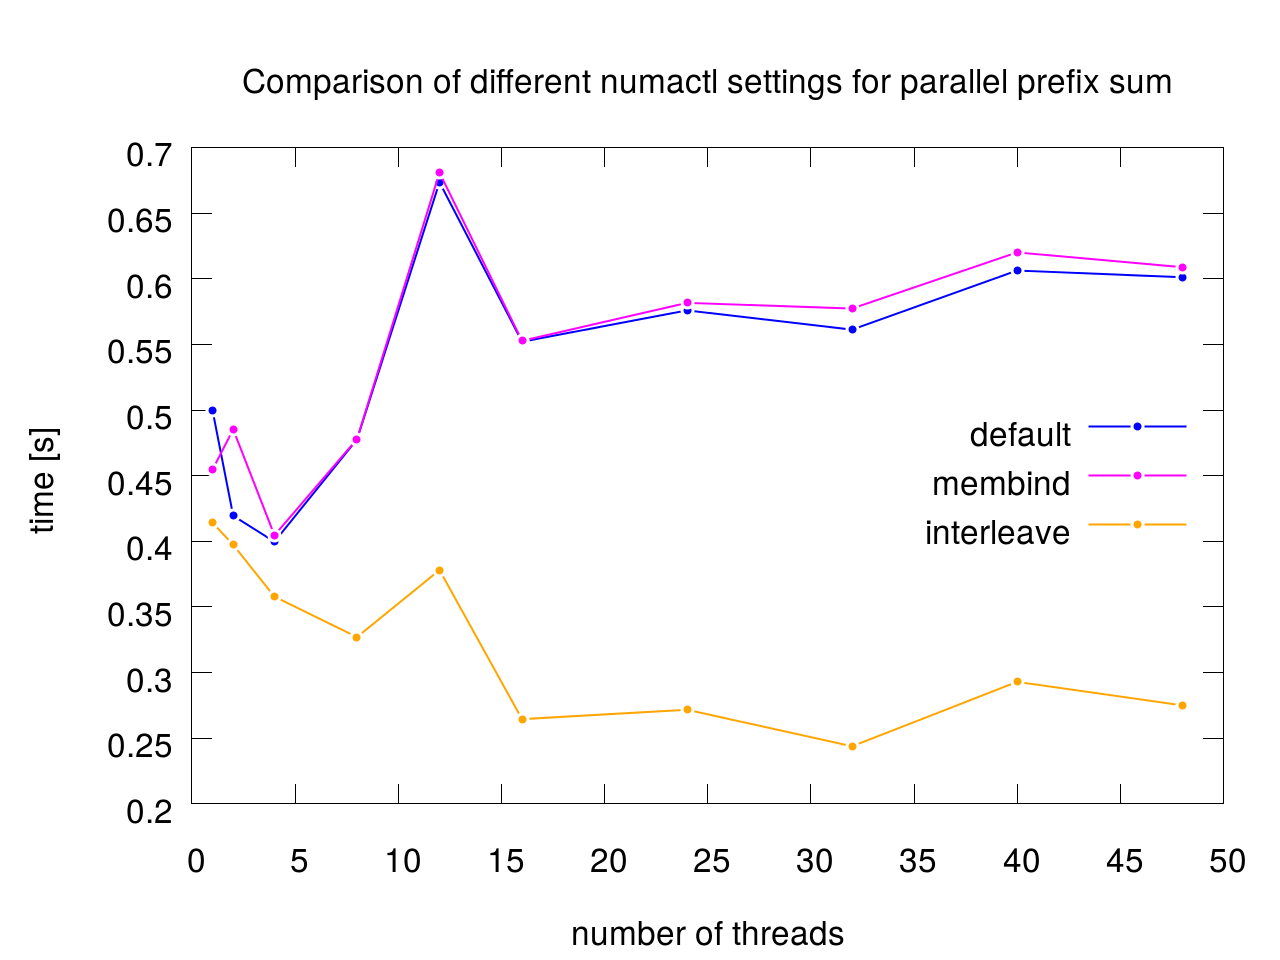
\includegraphics[width=0.8\textwidth]{comparison.png}
    \caption{Runtimes for the parallel prefix sum.}
    \label{fig:comparison}
\end{figure}

The fact that the results for the default and the membind configurations are mostly the same leads us to the conclusion that per default the memory is bind to one socket. Hence, one should enable interleave=all or similar options when running multi-threaded implementations as shown by the performance of this configuration. \\
All settings show a peak at about TC=12 which is the number of cores per die. This may be expected for the default and membind configurations, but not for the interleaved one. Since it makes usage of the distribution of the array different cores on different dies seem to be used... This remains unclear to us.

\end{homeworkProblem}

\clearpage
\end{document}
